\documentclass{beamer}
\usepackage{fontspec}
\usepackage{bibentry}
\usepackage{graphicx}

\setmainfont{Sarasa-Fixed-Slab-SC-Regular}
\setsansfont{HelveticaNeue}
\setbeamertemplate{frametitle}[default][center]

\mode<presentation> {

% The Beamer class comes with a number of default slide themes
% which change the colors and layouts of slides. Below this is a list
% of all the themes, uncomment each in turn to see what they look like.

\usetheme{default}
%\usetheme{AnnArbor}
%\usetheme{Antibes}
%\usetheme{Bergen}
%\usetheme{Berkeley}
%\usetheme{Berlin}
%\usetheme{Boadilla}
%\usetheme{CambridgeUS}
%\usetheme{Copenhagen}
%\usetheme{Darmstadt}
%\usetheme{Dresden}
%\usetheme{Frankfurt}
%\usetheme{Goettingen}
%\usetheme{Hannover}
%\usetheme{Ilmenau}
%\usetheme{JuanLesPins}
%\usetheme{Luebeck}
%\usetheme{Madrid}
%\usetheme{Malmoe}
%\usetheme{Marburg}
%\usetheme{Montpellier}
%\usetheme{PaloAlto}
%\usetheme{Pittsburgh}
%\usetheme{Rochester}
%\usetheme{Singapore}
%\usetheme{Szeged}
%\usetheme{Warsaw}

% As well as themes, the Beamer class has a number of color themes
% for any slide theme. Uncomment each of these in turn to see how it
% changes the colors of your current slide theme.

%\usecolortheme{albatross}
%\usecolortheme{beaver}
%\usecolortheme{beetle}
%\usecolortheme{crane}
%\usecolortheme{dolphin}
\usecolortheme{dove}
%\usecolortheme{fly}
%\usecolortheme{lily}
%\usecolortheme{orchid}
 %\usecolortheme{rose}
%\usecolortheme{seagull}
%\usecolortheme{seahorse}
%\usecolortheme{whale}
%\usecolortheme{wolverine}

%\setbeamertemplate{footline} % To remove the footer line in all slides uncomment this line
%\setbeamertemplate{footline}[page number] % To replace the footer line in all slides with a simple slide count uncomment this line

%\setbeamertemplate{navigation symbols}{} % To remove the navigation symbols from the bottom of all slides uncomment this line
}

\usepackage{graphicx} % Allows including images
\usepackage{booktabs} % Allows the use of \toprule, \midrule and \bottomrule in tables

%----------------------------------------------------------------------------------------
%	TITLE PAGE
%----------------------------------------------------------------------------------------

\title[Short title]{Privacy-Preserving Protocol Based On Bluetooth Encrypted Data Sharing} % The short title appears at the bottom of every slide, the full title is only on the title page

\author{ Wangzhihui Mei 2019124044\ Hongyi Huang 2019180029 \ Zijia He 2019124057 \ Chang Xu 2019180034\\ Tianyu Jin 2019180030 \ Zhanping Zhou 2019124060 \ Senmiao Liu 2019180036 \ Caiming Qian 2019124036} % Your name
\institute[JI] % Your institution as it will appear on the bottom of every slide, may be shorthand to save space
{
CCNU-UOW JI \\ % Your institution for the title page
\medskip
\textit{maywzh@gmail.com} % Your email address
}
\date{\today} % Date, can be changed to a custom date

\begin{document}

\begin{frame}
\titlepage % Print the title page as the first slide
\end{frame}

\begin{frame}
\frametitle{Overview} % Table of contents slide, comment this block out to remove it
\tableofcontents % Throughout your presentation, if you choose to use \section{} and \subsection{} commands, these will automatically be printed on this slide as an overview of your presentation
\end{frame}

%----------------------------------------------------------------------------------------
%	PRESENTATION SLIDES
%----------------------------------------------------------------------------------------

%------------------------------------------------
\section{Introduction}
\subsection{Background}
\begin{frame}
  \frametitle{Background}
  The pandemic of COVID-19 is devastating, which has caused global impact.

  The "health code", as a pass for returning personnel, records the individual’s health and takes the form of "green code", "red code", and "yellow code" to dynamically detect data. 

\end{frame}

\subsection{Requirement}
\begin{frame}
  \frametitle{Requirement}
  \begin{itemize}
    \item The personal information is hidden to server
    \item Location and time window of infected ones is possible
    \item Statistical data is available
    \item Information transferred between parties should be protected
  \end{itemize}

\end{frame}

%------------------------------------------------



%------------------------------------------------

\section{Protocol}
\subsection{Analysis}
\begin{frame}
  \frametitle{Analysis}
  \begin{itemize}
    \item Privacy should be kept on local device except for being infected
    \item All data transmission process should be encrypted
    \item The client is anonymous to other clients and servers
  \end{itemize}

\end{frame}
\subsection{Proposed Protocol}
\begin{frame}[allowframebreaks]
  \frametitle{Protocol}
  \begin{columns}[c]
  \column{.5\textwidth}
  \begin{itemize}
    \item Periodic Rolling Exposure Key(PREK)
    \item Interval Proximity Identifier Key(IPIK)
    \item Encrypted User Metadata Key(EUMK)
  \end{itemize}
  \column{.45\textwidth} % Left column and width
  \begin{figure}[]
    \centering
    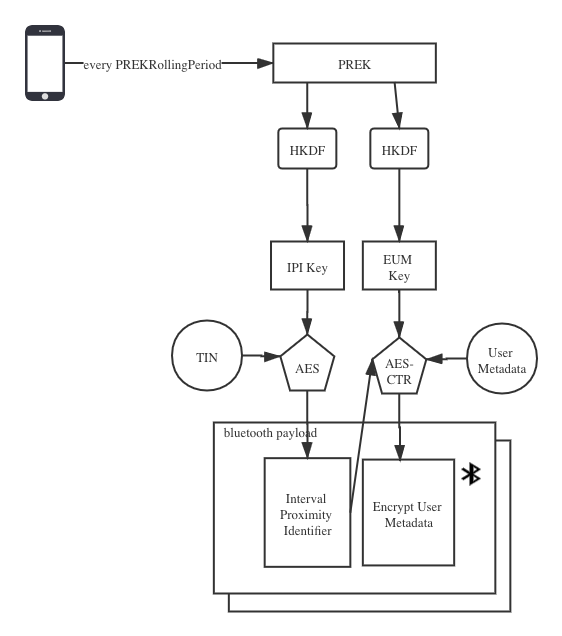
\includegraphics[height=1.3\textwidth]{figure/Tracking}
    \caption{Key generation and Encryption}
  \end{figure}
\end{columns}

\begin{figure}[]
  \centering
  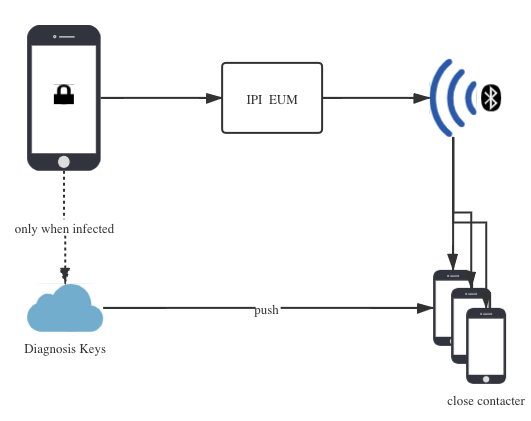
\includegraphics[height=0.6\textwidth]{figure/judge}
  \caption{Data transmission}
\end{figure}
\end{frame}

\begin{frame}
  \frametitle{Mathematic Details}
  \begin{columns}[c]
    \column{.5\textwidth}
    \small$$TIN(timestamp)\leftarrow timestamp/(60\times 15)$$
    
    $$i\leftarrow \lfloor TIN(timestamp)/PREKP\rfloor \times PREKP$$
    $$PREK_i\leftarrow CRNG(16)$$
    $$IPIK_i\leftarrow HKDF(PREKP_i,NULL,UTF8("IPIkey"), 16)$$
    $$IPI_{i,j}\leftarrow AES_{128}(RPIK_i,0||TIN_j)$$
    $$EUMK_i\leftarrow HKDF(PREK_i,NULL,UTF8("EUMKey"), 16)$$
    $$EUM_{i,j}\leftarrow AES_{128}-CTR(EUMK_i,IPI_{i,j},BLEMetadata)$$
    \column{.45\textwidth} % Left column and width
    \begin{figure}[]
      \centering
      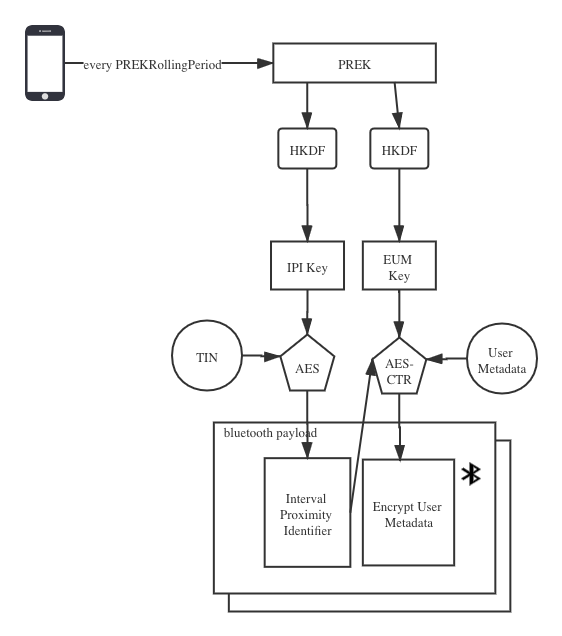
\includegraphics[height=1.3\textwidth]{figure/Tracking}
      \caption{Key generation and Encryption}
    \end{figure}
  \end{columns}

\end{frame}
\subsection{}

\section{Security and Functionalities}
\subsection{Security}
\begin{frame}
  \frametitle{Security}
  \begin{itemize}
    \item Only infector’s Periodic Rolling Exposure Key will upload to the cloud server
    \item The encrypted metadata cannot be decrypted without PREK
    \item Client-to-client communication is based on authenticated Bluetooth data transmission
  \end{itemize}

\end{frame}

\subsection{Functionalities}
\begin{frame}
  \frametitle{Functionalities}
  \begin{itemize}
    \item Data statistics is possible as the register data can be collected.
    \item Location and time windows of infected can be tracing.
  \end{itemize}

\end{frame}


\begin{frame}
\Huge{\centerline{The End}}
\end{frame}

%----------------------------------------------------------------------------------------

\end{document} 